\documentclass[mathserif,handout]{beamer}
%\documentclass{beamer}
\usetheme{metropolis}
\usepackage{amsmath,verbatim}
\usepackage{listings}
\usepackage[english]{babel}
%\usepackage{movie15}
\setbeamercovered{transparent}

\newcommand{\Deltap}{\ensuremath{\Delta^{\!+}}}
\newcommand{\trans}{\ensuremath{{}^\mathrm{T}}}
\newcommand{\eps}{\varepsilon}
\newcommand*{\approxdist}{\mathrel{\vcenter{\offinterlineskip
\vskip-.25ex\hbox{\hskip.55ex$\cdot$}\vskip-.25ex\hbox{$\sim$}
\vskip-.5ex\hbox{\hskip.55ex$\cdot$}}}}

% \lstMakeShortInline[language=myR]¬

\lstdefinelanguage{myR}
{
   language=R,
   otherkeywords={read.table, set.seed, head},
   deletekeywords={url,codes, t, dt, Call, formula,Q, R, on,by,hat,is,
col, set,start,end,deltat,zip},
   sensitive=true,
   breaklines=true,
   morecomment=[l]{\#},
   morestring=[b]",
   morestring=[b]',
   basicstyle =\ttfamily\small,
   keywordstyle=\bfseries,
   showtabs=false,
   showstringspaces=false,
   literate= {~}{$\sim$}{2},
   numberstyle=\sffamily\scriptsize,
   stepnumber=2
 }



\title{Discussion of: Unbiased MCMC with couplings}
\author{\textbf{\large Darren 
Wilkinson} \\
\url{@darrenjw}\\
\alert{\url{darrenjw.github.io}}\\
Newcastle University and The Alan Turing Institute\\}
\date{RSS, Errol Street, London\\11th December, 2019}

\begin{document}

\frame{\titlepage}

\frame{
  \frametitle{The big picture}
  \begin{itemize}
  \item blah
  \end{itemize}
Materials: \alert{\url{https://github.com/darrenjw/unbiased-mcmc}}
}

\frame{
  \frametitle{Coupled Metropolis chains (with offset of 1)}
\centerline{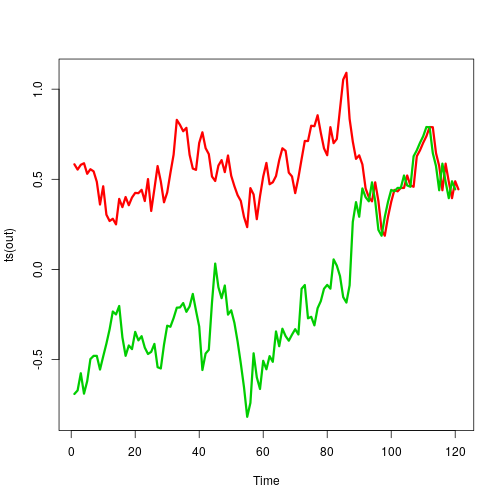
\includegraphics[height=0.95\textheight]{figs/coupled-mh}}
}

\frame{
  \frametitle{Coupled AR(1) chains}
\centerline{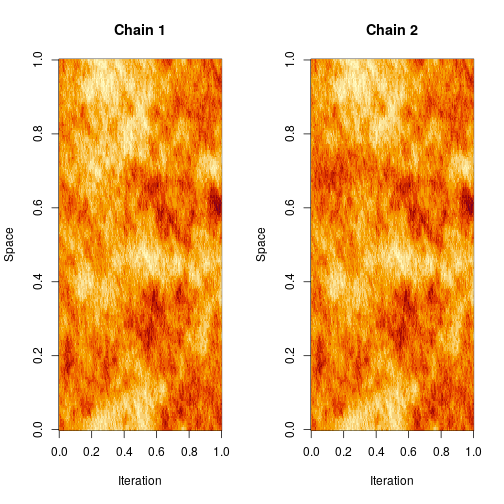
\includegraphics[height=0.95\textheight]{figs/ar1-chains}}
}

\frame{
  \frametitle{Coupled AR(1) variables}
\centerline{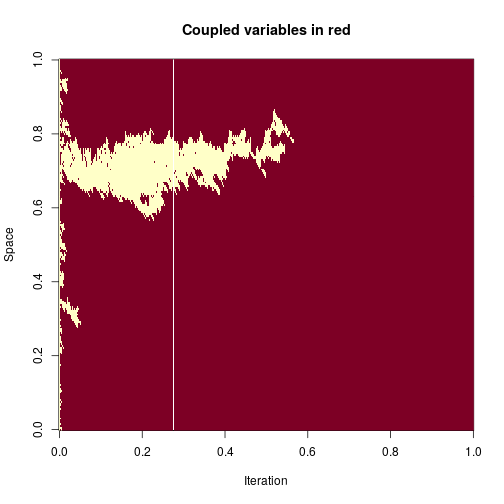
\includegraphics[height=0.95\textheight]{figs/ar1-coupled-1}}
}

\frame{
  \frametitle{Coupling behaviour for pairs of AR(1) chains}
\centerline{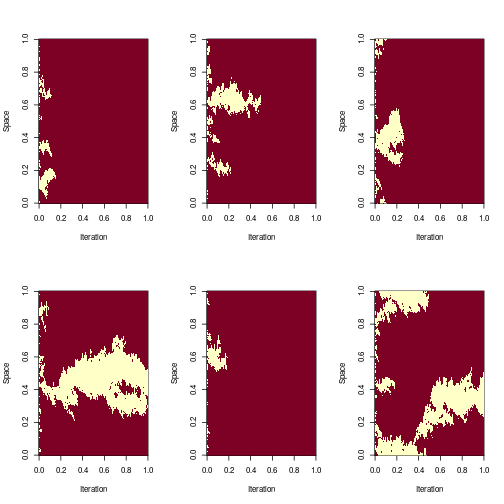
\includegraphics[height=0.95\textheight]{figs/ar1-coupled-6}}
}

\frame{
  \frametitle{Slide with movie}

}



\frame{
  \frametitle{In conclusion...}
  \begin{itemize}
  \item Good thing
  \item Less good thing
  \item Good thing
  \item Lots to discuss
  \item Propose vote of thanks
  \end{itemize}
Materials: \alert{\url{https://github.com/darrenjw/unbiased-mcmc}}
  
}


\end{document}
